\documentclass{article}


% if you need to pass options to natbib, use, e.g.:
%     \PassOptionsToPackage{numbers, compress}{natbib}
% before loading neurips_2023


% ready for submission
\usepackage[final]{neurips_2023}


% to compile a preprint version, e.g., for submission to arXiv, add add the
% [preprint] option:
%     \usepackage[preprint]{neurips_2023}


% to compile a camera-ready version, add the [final] option, e.g.:
%     \usepackage[final]{neurips_2023}


% to avoid loading the natbib package, add option nonatbib:
%    \usepackage[nonatbib]{neurips_2023}


\usepackage[utf8]{inputenc} % allow utf-8 input
\usepackage[T1]{fontenc}    % use 8-bit T1 fonts
\usepackage{hyperref}       % hyperlinks
\usepackage{url}            % simple URL typesetting
\usepackage{booktabs}       % professional-quality tables
\usepackage{amsfonts}       % blackboard math symbols
\usepackage{nicefrac}       % compact symbols for 1/2, etc.
\usepackage{microtype}      % microtypography
\usepackage{xcolor}         % colors
\usepackage{graphicx}
\usepackage{float}
\usepackage{amsmath}

% Title ideas: 
% A Blind Approach to Hyperspectral Deep Deconvolution
% Deep Learning for Hyperspectral Blind Deconvolution
% Deep Learning for Hyperspectral Deconvolution
% Hyperspectral Blind Deep Deconvolution
% Blind Deep Deconvolution for Snapshot Hyperspectral Images
% Deep Blind Deconvolution for Snapshot Hyperspectral Images
\title{Single-shot Hyperspectral Imaging via Deep Chromatic Aberration Deconvolution}

\author{%
   Corey Zheng \\
   College of Biomedical Engineering, Georgia Tech  \\
  % Address \\
   \text{czheng@gatech.edu} \\
   \AND
   Austin Barton \\
   Georgia Tech \\
  % Address \\
   \text{abarton40@gatech.edu} \\
   \And
   Mohammad Taher \\
   Georgia Tech \\
  % Address \\
   \text{mtaher3@gatech.edu} \\
   \And
   Abdulaziz Memesh \\
   Georgia Tech \\
  % Address \\
   \text{a.memesh@gatech.edu} \\
}


\begin{document}

\maketitle


\begin{abstract}
  This paper addresses the challenge of chromatic aberration in snapshot hyperspectral imaging, where the introduction of a third spectral dimension complicates encoding information into a two-dimensional detector plane. While traditional methods rely on scan-based approaches, our proposed method aims to enhance the quality of hyperspectral images by mitigating distortions inherent in snapshot acquisitions by leveraging a blind deconvolution approach with a U-Net neural network architecture for single-shot hyperspectral imaging. Our approach allows real-time correction without the need for complex scanning mechanisms nor knowledge of point spread functions. Through experimental validation, we demonstrate the efficacy of our method in preserving image structure and spectral composition information, contributing to improved imaging throughput and simplified hardware requirements. Our best performing model is capable of restoring spectral information among test data, even in pixel locations with highly varying wavelength intensities, while deblurring and restoring an approximation of the latent sharp image. Our paper represents a simple yet effective approach to circumventing issues in snapshot hyperspectral imaging, providing a practical solution for applications in medical imaging, agriculture, materials identification, and geological surveillance.
\end{abstract}


\section{Introduction}
Hyperspectral imaging is a highly important imaging modality, with the ability to capture the unique wavelength emission and reflectance spectra of objects within the field of view. For every spatial pixel within a hyperspectral image, the captured spectrum is a superposition of all unique spectra produced by molecules within the spatial region, and thus is a measure of the chemical composition at each spatial location within the field of view (FOV). This higher-dimensional spectral information has therefore enabled major strides in medical imaging \cite{lu2014medical}, agriculture \cite{lu2020recent}, materials identification \cite{dong2019review}, geological surveillance \cite{peyghambari2021hyperspectral}, and more.  

However, hyperspectral images have been difficult to acquire, as their three-dimensional nature (two spatial dimensions and a spectral dimension) cannot be fully represented on electronic image sensors which feature two-dimensional arrays of pixels. Traditional hyperspectral imaging approaches are scan-based, scanning through either one spatial dimension such as pushbroom approaches, or one spectral dimension by utilizing a series of filters \cite{gao2015optical}. Such approaches limit the imaging throughput speed and also require more complex imaging setups that involving parts such as scanning galvo mirrors, acousto-optical deflectors, filters, or acousto-optical filters.

Thus, a major research interest is \textit{snapshot hyperspectral} imaging, in which the full hyperspectral volume can be captured in a single image frame, greatly increasing the acquisition throughput and eliminating the need for complex scanning components. Early snapshot hyperspectral imaging began by mapping slices of the hyperspectral volume to different spatial positions on a two-dimensional camera detector. Approaches in this category include Computed Tomography Imaging Spectrometers (CTIS) \cite{FORD2001986} and Integral Field Spectrography (IFS) \cite{allington2006basic}. These mapping approaches necessitate a trade-off due to their subdivision of the imaging sensor, requiring a reduction of either the field of view (FOV) or resolution in order to fit both the spatial image and spectral components onto a sensor with the same number of pixels.

Motivated by this inherent compromise, various computational based approaches aimed at reconstructing the hyperspectral information without subdivisions of the imaging field have been introduced. In particular, \textit{chromatic aberration} approaches that take advantage of a uniquely varying wavelength dependent point-spread function (PSF) have been used to encode spectral information into the spatial blur of an image \cite{zhan2019hyperspectral,baek2021single,jeon2019compact} in a similar vein as depth-from-defocus approaches \cite{ming2021deep}.

Following this research area, we present our work: Single-shot Hyperspectral Imaging via Deep
Chromatic Aberration Deconvolution. We explore using deep U-net networks to perform hyperspectral volume reconstruction from a single chromatically-aberrated monochromatic image. In particular, our contributions compared to related works are (1) independence of costly and customized diffraction masks that require lithography approaches, lowering the barrier to entry and presenting a more accessible snapshot hyperspectral imaging solution, (2) requires only a single monochromatic image at an infinity focus, rather than a set of images at different foci for improved imaging throughput, and (3) usage of a deep network rather than iterative reconstruction process, improving forward model processing speed. We envision these advancements will guide the development of lower-cost, simpler snapshot hyperspectral imaging systems for wide applications.

\section{Related Works}
In this section we review approaches towards snapshot hyperspectral imaging.

\subsection{CTIS}
Snapshot hyperspectral imaging began with the introduction of Computed Tomography Imaging Spectrometers (CTIS) \cite{FORD2001986}. In this approach, an additional dispersive element is introduced into the imaging system, essentially splitting an incoming image into multiple tiled copies, with each copy exhibiting a different amount of radial chromatic blur. This follows the same concept as lightfield imaging \cite{guo2019fourier}\cite{broxton2013wave} but utilizes diffraction orders produced from chromaticity rather than depth. In a sense, such an approach could also be considered a class of \textit{chromatic aberration} approaches. However, it is differentiated from other chromatic aberration approaches by key disadvantages: (1) The authors utilize an iterative reconstruction algorithm (MART) in order to recover the final image, but this algorithm is time consuming and requires measurement of multiple calibration matrices. (2) The usage of a dispersive element to create multiple tiled copies (e.g. 7×7) results in a reduction in the field of view of the image due to the subdivision of the camera sensor area.

\subsection{Bioinspired Chromatic Vision Blur}
Unlike mammalian eyes which have separate neuroreceptors with sensitivities tailored towards different wavelengths (primarily red, blue, green), cephalopod eyes have broadband neuroreceptors sensitive to all wavelengths. Yet, these animals can still discriminate colors through recognition of the form of the chromatic blur they produce. Inspired by this, Zhan et al. utilized a chromatic aberration system coupled with an SVD-based iterative reconstruction algorithm to restore hyperspectral stacks from monochromatic blurred images \cite{zhan2019hyperspectral}. However, the authors had to utilize 3 images of the same object at different distances in order to achieve their results, meaning a compromise between imaging speed, FOV, or resolution is necessary to apply this approach in the field, as three separate images must be acquired for a single reduction. Furthermore, the data the authors demonstrated their results on was extremely well-behaved - the authors only showed reconstruction on images that contained single-peak gaussian-esq spectra, rather than more realistic scenarios, indicating that there may have been potential trouble with separability in their approach via classical iterative deconvolution.

\subsection{Diffracted Rotation and End-to-End Optimization}
Utilizing dispersion engineering, it is possible to create custom optical elements with controllable chromatic blurring patterns. Jeon et al. \cite{jeon2019compact} formulated an approach, designing a custom diffractive optical element (DOE) that creates a triple-helix point-spread function which rotates based on the wavelength. Thus, the authors were able to increase the separability of the chromatically-aberrated images by eliminating the radial symmetry of their blur kernels. They combined this with a learned unrolled network architecture based on U-net, combined with an iterative algorithm to reconstruct hyperspectral stacks. The author also later followed on this work with a joint hyperspectral-and-depth reconstruction from a single monochromatic image using end-to-end optical optimization \cite{baek2021single}. In this approach, end-to-end optimization was performed by implemented a differentiable optics simulation prior to a deep learning U-net and optimizing both systems jointly \cite{chakrabarti2016learning}\cite{zou2023advanced}, resulting in a co-optimized PSF encoding of spectral and depth information that could be best reconstructed by the deep U-net. Both of these works showed promising results, however, in both cases, a complex DOE was fabricated via lithographic means \cite{poleshchuk2010fabrication}, which restricts accessibility.

\section{Methods}

\subsection{Image formation model}

As a basis for the optical physics of the system, our image formation model utilizes the following assumptions:
\begin{enumerate}
    \item The PSF is \textit{spatially invariant}.
    \item The camera operates in the \textit{hyperfocal range} where all objects are in-focus \cite{kingslake1992optics}:
    \begin{equation}
        PSF(\lambda,z) = PSF(\lambda) 
    \end{equation}
    \item The camera has uniform sensitivity across the entire light spectrum.
\end{enumerate}

Assumption (1) is frequently utilized in optical imaging fields, as with it an image can be conveniently described as the convolution of an underlying object with the PSF \cite{goodman2005introduction}:

\begin{equation}
    I(\lambda) = g(\lambda) \ast PSF(\lambda)
\end{equation}

Where $I(\lambda)$ is the captured image at some wavelength and $g(\lambda)$ is the underlying unblurred object at some wavelength. Given a monochromatic camera that is equally sensitive to all wavelengths (assumption 3), the object as imaged by our chromatic aberration optical system can be simulated as:

\begin{equation}
    I = \int_\lambda g(\lambda) \ast PSF(\lambda)
\end{equation}

This set of assumptions are are often employed in optical imaging to simplify the computational process, being similarly applied in a related work \cite{jeon2019compact}. Our optical system is shown in Figure \ref{fig:opticalsystem}, along with every band of the chromatic PSF. Additional information about the parameters of the optical system are presented in Appendix \ref{sec:appendixOptical}.

\begin{figure}
    \centering
    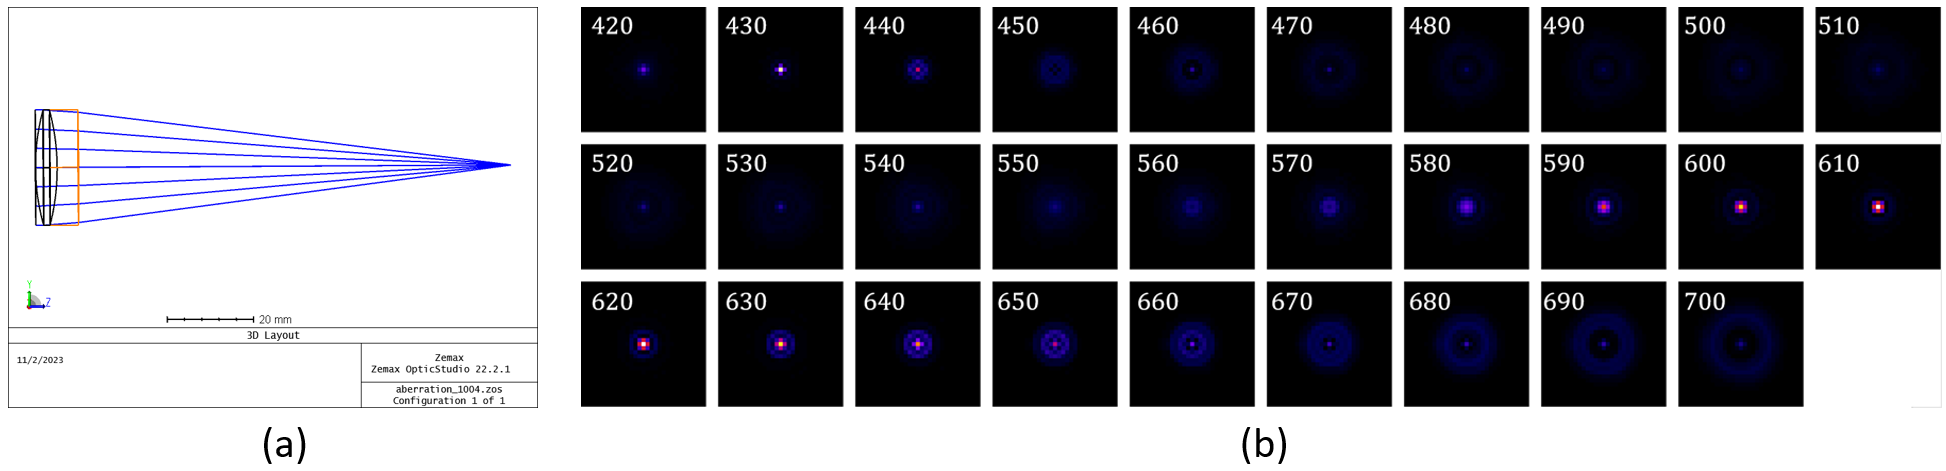
\includegraphics[width=\textwidth]{figs/opticalsystem.png}
    \caption{Optical imaging system. \textbf{(a)} Ray tracing simulation of chromatic aberration imaging system with singular doublet lens. \textbf{(b)} Chromatic PSF in every wavelength band generated from simulated optical system.}
    \label{fig:opticalsystem}
\end{figure}

\subsection{Dataset}
We are utilizing a combination of 5 hyperspectral datasets \cite{CAVE_0293}\cite{chakrabarti2011statistics}\cite{arad_and_ben_shahar_2016_ECCV}\cite{DeepCASSI:SIGA:2017}\cite{farrell2003simulation}, which results in a total of 394 unique hyperspectral images covering objects including human faces, architecture, household objects, landscapes, and more.

\subsection{Data Preprocessing}
The model flowchart is depicted in Figure \ref{fig:mainflow}. For model training, we synthesize the input monochromatic image by simulating the sensor image of the chromatically aberrated imaging system described above. All data from the 5 hyperspectral datasets were cropped to a common spectral range of 420-700nm, with steps of 10nm bands. Images were resized to a height of 512 pixels, maintaining the same aspect ratio, in order to compensate for variation in image resolutions and maintain feature density to minimize the changes of sampling low-feature empty patches. To synthesize blurred images simulating a chromatically-aberrated optical imaging system, each spectral band was convolved with the corresponding PSF and summed as described in the image formation model, resulting in a monochromatic blurred image representing the image captured by our chromatic aberration imaging system. Finally, we randomly sampled 16 128×128 pixel patches from each monochromatic image and extracted the corresponding 29×128×128 pixel hyperspectral volume to form input and ground truth pairs, respectively. The resultant dataset consists of 6304 patches, with no augmentations (additional discussion provided in Section \ref{sec:resourcelimitations}).

\begin{figure}
    \centering
    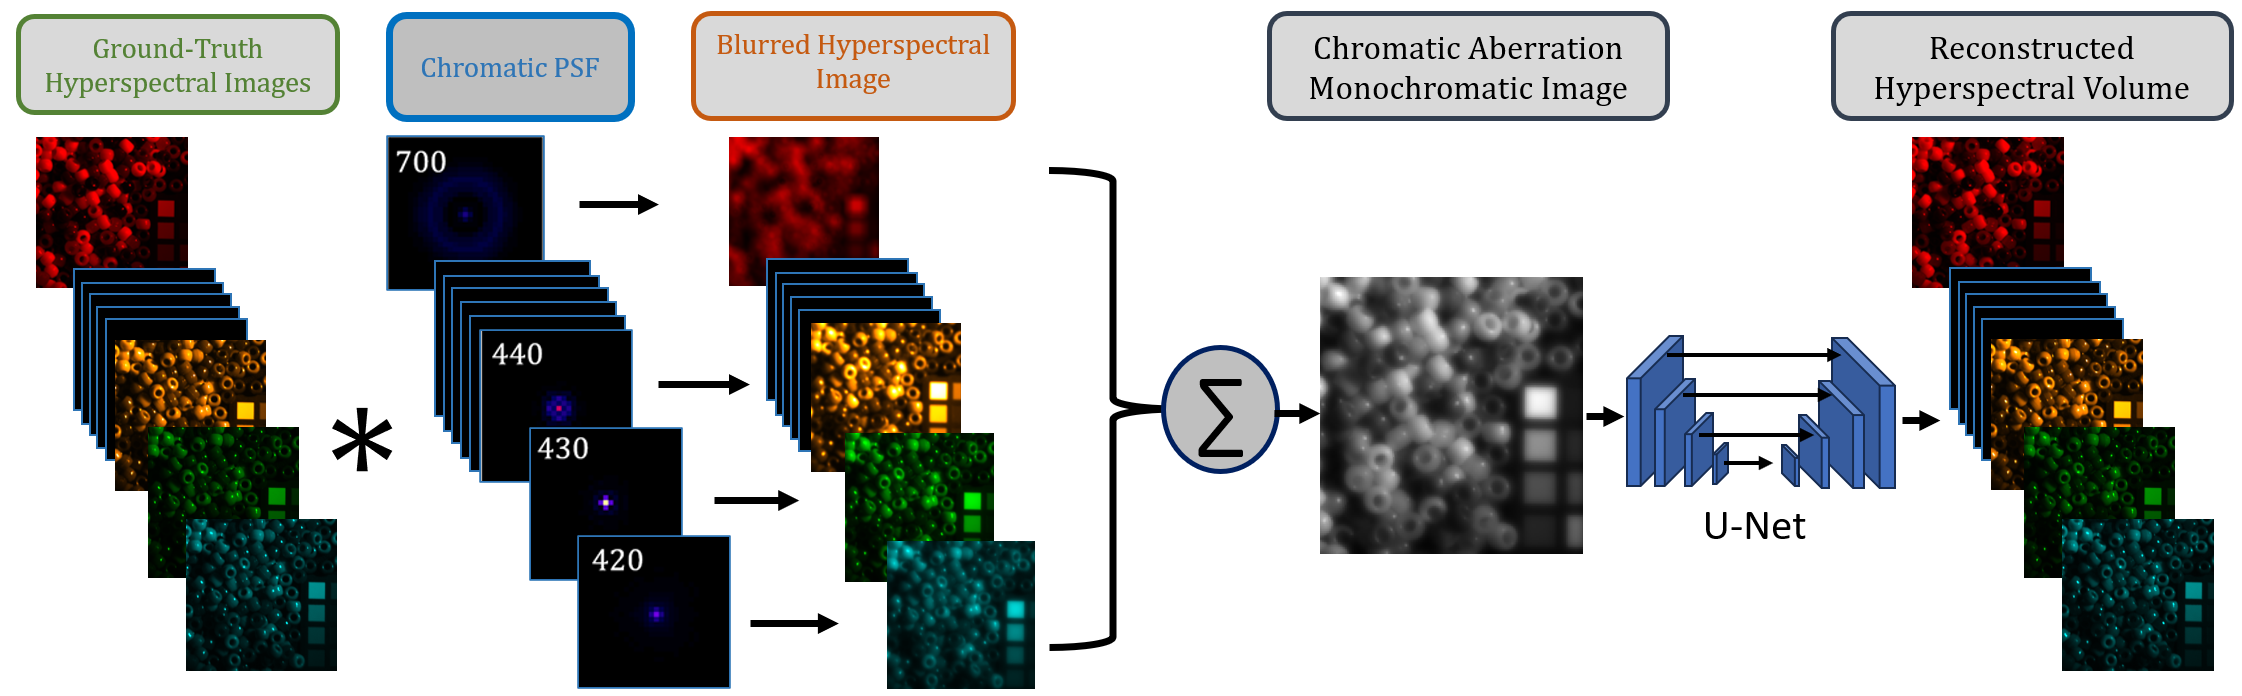
\includegraphics[width=\textwidth]{figs/mainflow.png}
    \caption{Main model flowchart. Chromatic aberration data is synthesized from ground truth data combined with simulated chromatic PSFs as an input to the deep U-net model for hyperspectral volume reconstruction.}
    \label{fig:mainflow}
\end{figure}


\subsection{U-Net Architecture}
To solve this task, we're using the U-Net, a deep convolutional neural network model developed for biomedical image segmentation by Ronneberger et al. \cite{Ronneberger_2018}. A U-Net model essentially acts as an Encoder-Decoder Convolutional Neural Network. There's the encoding path that shrinks the image and increases the number of channels to bottleneck the input, then the decoding path which expands the image and decreases the number of channels. It's similar to an autoencoder, but with skip connections from the encoded representations concatenated to the decoded outputs at each upsampling step.

One of the defining characteristics of U-Nets is localization, where every outputted pixel can be measured against a target value relative to the input. Ronneberger et al \cite{Ronneberger_2018} found that their U-Net outperformed the existing method of patchwise classification via CNNs and drastically improved the computational costs in achieving their task. Therefore, we decided to use a U-Net model due to its high performance and low complexity. 

The model inputs a 1×128×128 pixel chromatically aberrated monochromatic image synthesized as described previously, and outputs a 29×128×128 hyperspectral volume in which each channel represents a 10nm wavelength band from 420-700nm. We implement two different architectures, depicted in Figure \ref{fig:Unet_model}.


\begin{figure}
  \centering
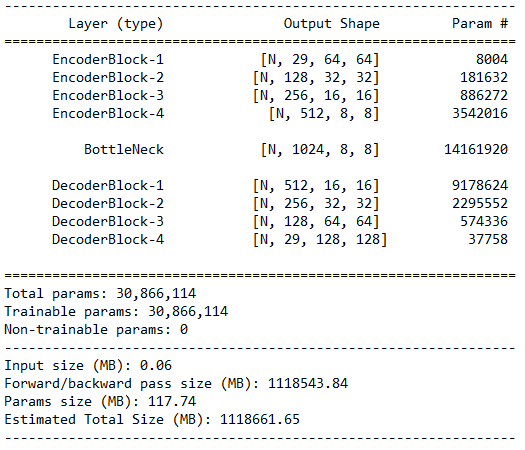
\includegraphics[width=\textwidth]{figs/model/model_summary_shortened.png}
  \caption{Model Summary}
  \label{fig:Unet_model}
\end{figure}


\subsection{Objective Function}
We want to minimize the difference of the spectral information between the output and ground truth images as well as restore perceptual quality. Therefore, the objective functions we experiment with are Structural Similarity Index Measure (SSIM) and Mean Squared Error (MSE). SSIM is a metric for image comparisons that compares the overall shapes and patterns, while MSE focuses on the raw pixel value differences \cite{Brunet_Vrscay_Wang_2011}. MSE can also be represented as the peak signal-to-noise ratio (PSNR), which accounts for differences in data type representations.

An underlying issue that MSE has in the context of image restoration is the fact that many perceptually different restored images can correspond to one MSE value. Because our problem is taking hyperspectral images that are corrupted by chromatic aberration and restoring them to their corresponding latent sharp images, it is possible that deblurred images outputted by our model may have low MSE but perceptually poor quality. Because of this, we experiment with a combination of MSE and SSIM as an objective function. Details of the mathematical formulation and conceptual explanations are found in \ref{subsec:appendix_ssim} and \cite{Brunet_Vrscay_Wang_2011}. Note SSIM indicates high structural similarity for higher values. Hence, we formulate our SSIM loss function as $1 - $SSIM.

\subsection{Baseline Comparison - Richardson-Lucy Deconvolution}
Richardson-Lucy (RL) deconvolution is a classical iterative procedure for recovering an unblurred image from a blurred image with a known PSF imaging system \cite{lucy1974iterative}\cite{richardson1972bayesian}. It can be considered a baseline approach for any sort of image deblurring. In the case that RL deconvolution is used to project a two-dimensional image back into a 3-dimensional underlying image by means of a 3D PSF (ie, depth varying PSF), RL deconvolution follows the form \cite{broxton2013wave}\cite{guo2019fourier}:

\begin{equation}
    g(z)^{k+1} = g(z)^{k} \cdot \left(\frac{O}{\sum_{z} \text{PSF}(z) \ast g(z)^{k} } \ast \text{PSF'}(z)\right)\text{for all z}
    \label{eq:RL}
\end{equation}

Where the $g^k$ is the underlying 3D volume and each slice of $g$ can be computed according to the RL update rule above. Here, the forward projection has been modified, projecting a 3D volume $g$ into the 2D image space via superposition of the convolution of each slice with its corresponding slice of the 3D PSF. In the case of hyperspectral images, the $z$ dimension can simply be replaced with the wavelength dimension $\lambda$. We consider RL deconvolution using 15 iterations as a baseline approach towards solving hyperspectral deconvolution and compare the results of our deep network against it. Additional details of implementation and optimization of RL deconvolution hyperparameters is discussed in the Appendix \ref{sec:appendixRL}.

\subsection{Experimental Setup}
We implemented the U-Net architectures in Python using the PyTorch deep learning platform. Models were trained for 1000 epochs, and the epoch which resulted in the lowest validation set loss was considered to be the best model and saved for final analysis. Training required approximately 8-9 hours on a workstation with a NVIDIA Quadro A4000 with 16GB VRAM and an Intel(R) Xeon(R) W-2145 CPU @ 3.70GHz with 512GB RAM. We conducted experiments involving varied model hyperparameters and architectures, as shown in Table \ref{hyperparams}. In-depth architectures are presented in Table \ref{fig:Unet_model}.

\begin{table}
  \caption{Experimental Hyperparameters}
  \label{hyperparams}
  \centering
  \resizebox{\textwidth}{!}{%
  \begin{tabular}{llll}
    \toprule
    Experiment & Loss Function & Optimizer & Learning Rate\\
    \midrule
    HyperUnet & MSE & Adam & 0.01    \\
    HyperUnet\textsubscript{LR} & MSE & Adam & [0.1, 0.01, 0.001] at epochs [0,200,600]    \\
    HyperUnet\textsubscript{SSIM} & MSE + SSIM & Adam & [0.1, 0.01, 0.001] at epochs [0, 200, 600]    \\
    HyperUnet_{Reduced} & MSE & Adam & [0.1, 0.01, 0.001] at epochs [0, 200, 600] \\
    \bottomrule
  \end{tabular}}
\end{table}

\section{Results}
\label{sec:results}



\subsection{Main Findings}
\label{sec:main-findings}
\begin{table}
    \caption{Loss comparison between our models and published hyperspectral imaging approaches}
    \label{Results}
    \centering
    \begin{tabular}{lllll}
    \toprule
    Model & PSNR(dB) & SSIM \\
    \midrule
    Baek et al.\cite{baek2017compact} & 27.96 & 0.75 \\
    Jeon et al.\cite{jeon2019compact} & 28.81 & \textbf{0.81} \\
    Baek et al.\cite{baek2021single} & \textbf{29.31} & \textbf{0.81} \\
    \midrule
    HyperUnet & \textbf{25.029} & 0.8681 \\
    HyperUnet\textsubscript{LR} & 24.945 & \textbf{0.8991} \\
    HyperUnet\textsubscript{SSIM} & 14.887 & 0.5187 \\
    HyperUnet\textsubscript{Reduced} & 22.292 & 0.7870 \\
    Richardson-Lucy Deconvolution & 14.713 & 0.8615 \\
    \bottomrule
    \end{tabular}
\end{table}

The loss of each network variation is presented in Table \ref{Results}. Of our models, HyperUnet and HyperUnet\textsubscript{LR} resulted in the best performance according to different metrics (PSNR, SSIM), respectively. Compared to other state-of-the art snapshot hyperspectral imaging methods, the absolute error (PSNR) was worse, but interestingly, our two top models had a lower SSIM loss compared to these approaches. This may indicate that custom dispersive elements utilized in previous approaches to create complex PSFs results in additional image aberrations that, though minimize the MSE, also result in a loss of the overall structure of the reconstructed volumes. In all cases, our deep models outperformed Richardson-Lucy deconvolution (Appendix \ref{appendix:RL}, Supplementary Figure \ref{fig:RLCompare}), which demonstrated an inability to perform spectral discrimination with the loss of multiple color channels.

Further analysis of test set sample reconstructions from both HyperUnet and HyperUnet\textsubscript{LR} revealed that, although HyperUnet\textsubscript{LR} has similar MSE and PSNR results to HyperUnet, HyperUnet\textsubscript{LR} failed to accurately recover crucial spectral information (\ref{fig:hyperunet_lr_beads}) in comparison to HyperUnet (\ref{fig:HyperUnet_results}). While HyperUnet\textsubscript{LR} obtained predictions that minimized SSIM\textsubscript{Loss} more by a considerable margin, the qualitative difference in deblurring is almost negligible and the spectral recovery was significantly worse than HyperUnet. Thus, HyperUnet was selected as the best network of the different experiments.

Spectral profiles are shown in Figure \ref{fig:HyperUnet_results}. Extracted spectra from spatial points in the image showed remarkable agreement between the predicted and ground truth spectrum, not just for mono-peak spectra as (Beads, pixel 3), but also for varied spectra with multiple local minima (Outdoors, pixel 3). Furthermore, our model shows a clear spatial deblurring effect as evidenced Figure ?.

\subsection{Limitations}
\subsubsection{Training Instability and PSF Degeneracy}
Instability of the network was a major factor towards model failure modes. With only variation of the hyperparameters, we found that the non-reduced HyperUnet would fail, typically by losing several wavelength bands (Appendix \ref{fig:degeneration_mode}). Typical failure modes manifested in gradient explosion during training (Appendix \ref{fig:UnetLR_grads}, \ref{fig:UnetSSIM_grads}). However, even after implementing gradient norm clipping, we still encountered mode collapse by losing wavelength bands, indicating a particularly ill-posed separation of these channels.

There exists a practical upper bound on retained information in such an image deblurring model. Observing the point-spread functions ---


Because we are taking in a monochromatic blurred image that consists of a superposition of all bands of light within the range as well as their respective blurring kernels, the unique structure of the point spread functions can be lost in sections of the image where pixel blurring effects overlap. This would mean that the underlying relationship between the blurring effect and spectral information would be lost and hence, impossible to recover.


\subsubsection{MSE+SSIM Objective Function Issues} 
The HyperUnet\textsubscript{SSIM} model showed highly unstable training from adding the second loss metric (SSIM) to the objective function and resulted in mode collapse. Specifically, the network effectively shrank pixel intensities of certain bands to $0$ and focused on outputting and correcting other bands (as seen in Figure \ref{fig:degeneration_mode}). Table \ref{Results} shows that this model with SSIM added into the objective function with MSE ended up resulting in a higher SSIM loss despite the model's objective function including SSIM loss.

\subsubsection{Overfitting}
Each model suffered from overfitting with the most extreme cases in the HyperUnet and HyperUnet\textsubscript{LR} (loss curves for each model are shown in the Figures \ref{fig:HyperUnet_results}, \ref{fig:loss_curve_HyperNet_model}, \ref{fig:loss_curve_HyperNetLR_model}, \ref{fig:loss_curve_UnetSSIM_model}, \ref{fig:loss_curve_ReducedUnet_model}). We experimented with reducing the architecture size, while fixing all other hyperparameters, to combat this overfitting issue and found that although it slightly reduced the overfitting, it performed much worse. We discuss this choice for experimentation and potential implications in Section \ref{sec:discussion}.

\begin{figure}[!h]
\centering
\includegraphics[width=\textwidth]{figs/hyperunet_consolidated_figure.png}
    \caption{Results from the the fully trained HyperUnet model. Pseudo-RGB ground truth and predicted images on four different images belonging to the test dataset are shown with markings for selected pixel coordinates for spectral plots (far left, top to bottom). Spectral plots comparing ground truth and predicted wavelength intensities for corresponding pixel coordinates (middle, top to bottom). In the top right is the model's training and validation loss curves. In the bottom right is a comparison of the model's performance in predicted spectral information between epoch 200 and the best model obtained after epoch 900.}
    \label{fig:HyperUnet_results}
\end{figure}

\subsubsection{Time and Computing Resources}
\label{sec:resourcelimitations}
Each model took approximately $8$ hours to train over 1000 epochs. With the deadlines of the project, experimentation of different models and hyperparameters was limited. For this reason, augmentations were also not utilized. Because the PSFs are radially asymmetric, all augmentations would have to be applied \textit{prior} to image convolutions, which would greatly increase processing time, and was not implemented for this work.

\section{Discussion}
\label{sec:discussion}
\subsection{Interpretation of Results}
We demonstrate an effective blind approach to deconvolution via deep learning in our best performing model, \text{HyperUnet}. However, in general, training these models is highly unstable and sensitive to the initialization of the model. Compared to other works, our model does not utilize customized DOEs which result in complex structured PSFs, nor does it utilize stacks of input images of varying focal lengths. In this sense, our approach enables far more accessible snapshot hyperspectral imaging with a higher theoretical throughput. As a trade-off, our model appears to also be far less \textit{separable}. Compared with customized structured PSFs, our PSFs have lower amounts of asymmetry and further possess self-similarity in different wavelength bands, which may contribute to the failure modes of the model, destroying one channel in any pair of two wavelength bands that have similar PSF structures. Furthermore, unlike other works which introduced multiple focal plane images to effectively construct four-dimensional PSFs (2D spatial structure, focal depth, and wavelength) to increase separability, our work relies on a single image. Thus, in conclusion, our approach boasts higher imaging efficiency and accessibility, but in doing so, increases the ill-posedness of the inverse problem making it unstable for training. This may limit real-world implementation, when not all the optical assumptions of the system are satisfied.

\subsection{Implications and Applications}
Our approach allows real-time correction without the need for complex scanning mechanisms nor knowledge of point spread functions. Through experimental validation, we demonstrate the efficacy of our method in preserving image structure and spectral composition information. This method can contribute to improved imaging throughput and simplified hardware requirements.

Applications such as medical imaging, agriculture, materials identification, and geological surveillance rely on hyperspectral imaging for a variety of reasons. All of them share a common need to be able to identify chemical composition. Chemical compositions can be studied and identified through sufficient spectral information. Issues with snapshot hyperspectral imaging complicates this. However, we demonstrate effective methods in being able to recover crucial spectral information and the latent sharp image without the need for the knowledge of the point spread functions of the optical lenses.

\subsection{Next Steps}
Although we were able to produce a model highly capable of our deconvolution task, we failed to make improvements upon the best HyperUnet model and we expect that reproducibility on different datasets would be quite difficult due to how sensitive the models were to the initialization of weights. Additionally, we found that our models consistently overfit the training data, even in the best performing network, demonstrating a need for further experimentation. Due to limited time and resources, we opted to experiment with a reduced architecture, the ReducedUnet, which ended up performing worse. This illustrates that it is likely that the overfitting is not due to how large the model is and opens up work for further experimentation on more sophisticated and properly tuned architectures for this task. Furthermore, as we suspect the form of the PSF to be highly involved in the failure modes of the network, investigation into asymmetric PSFs without self-similarity that can be achieved with conventional optics rather than custom DOEs will also be important towards enabling accessible snapshot hyperspectral imaging. 

\section{Acknowledgements}
We would like to thank Professor Danfei Xu and all of the teaching faculty for CS 7643 Deep Learning, Fall 2023 at Georgia Tech.

\section{Code Repository}
All code for this project was implemented in Python and is open-source. Code repository can be access through this link: \href{https://github.com/abarton51/Hyperspectral-Deep-Deconvolution}{https://github.com/abarton51/Hyperspectral-Deep-Deconvolution}.

\section{Team Contributions}
\begin{tabular}{p{0.15\linewidth} | p{0.8\linewidth}}
    \toprule
    Corey Zheng & Theoretical background, optical simulation \& image formation model, dataset collection \& dataset synthesis, RL-deconvolution baseline comparison, model training framework, model evaluation framework \& metric generation, hyperparameter experimentation, network failure modes \& debugging, figure generation, manuscript\\
    \midrule
    Austin Barton & Figure analysis, figure generation, dataloader implementation, pixel comparison procedure \& implementation, SSIM implementation, custom loss function implementation, results \& analysis, manuscript \\
    \midrule
    Mohammad Taher & \\
    \midrule
    Abdulaziz Memesh & \\
    \bottomrule
\end{tabular}

\bibliographystyle{plainnat}
\bibliography{paper/ref}

\newpage
\appendix
\section{Supplementary Material}
\label{sec:appendix}
\subsection{Optical System}
\label{sec:appendixOptical}
The optical system is a simple single lens design. The aperture is F/4, with a doublet lens with a 100mm focal distance at 525nm. Doublet lens is comprised of a positive asphere of N-BK7 crown glass, with a spherical concave flint component using N-F2 glass. The system was designed in Ansys Zemax OpticStudio.

\subsection{Structural Similaity Index Measure}
\label{subsec:appendix_ssim}
SSIM achieves accurate image comparisons without allowing the overall structure of the image to change, so the network can't recreate an image that's completely different. This metric's goal is to accurately measure the perceptual quality of an image using a combination similarity
measurements between each image's luminance, contrast, and structure. Luminance is described by a function of each image's the mean pixel value, contrast is described by a function of each image's standard deviation, and structure is a function of the centered and normalized pixel values. Something important to note is that the range of SSIM is $[-1, 1]$ with larger output values corresponding to greater similarity. Therefore, we formulate our "SSIM Loss" function as
\begin{equation}
    \text{SSIM}_{Loss} = 1 - \text{SSIM}
\end{equation}

which has a range of $[0, 2]$, with high similarity corresponding to lower values. However, this may cause the model to prioritize improving structural similarity to the point where it fails to restore spectral information. On the other hand, MSE can severely penalize any pixel differences, which may ensure that we don't lose as much information, specifically spectral information. 

We experimented with a combination of both of these since our problem requires both image deblurring and spectral information recovering.

\subsection{Richardson-Lucy Deconvolution Details}
\label{appendix:RL}
Originally, Richardson-Lucy (RL) deconvolution was an iterative procedure for two-dimensional image deblurring with a known PSF \cite{lucy1974iterative}\cite{richardson1972bayesian}, and widely applied as a standard method towards image deblurring. The RL deconvolution scheme is as follows for a two-dimensional image and two-dimensional known PSF:

\begin{equation}
    g^{k+1} = g^{k} \cdot \left(\frac{O}{\text{PSF} \ast g^{k} } \ast \text{PSF'}\right)
\end{equation}

Where $O$ is the captured blurred image, $g^{k}$ is the estimate of the unblurred image at iteration $k$, PSF is the point-spread function of the system, and PSF' is the point spread function of the system rotated by 180 degrees. 

In the case that RL deconvolution is used to project a two-dimensional image back into a 3-dimensional underlying image by means of a 3D PSF (ie, depth varying PSF), RL deconvolution follows a slightly modified originating from optical tomography \cite{broxton2013wave}\cite{guo2019fourier}, maintaining the structure of forward (into the blurred image space) and backwards (into the underlying space) projections, presented in Equation \ref{eq:RL}.

We coded a hyperspectral RL deconvolution algorithm. As shown in Supplementary Figure \ref{fig:RL2DCompare}, our modified 3D RL deconvolution performs similarly to classical 2D RL deconvolution on a standard blurred 2D image. Because RL deconvolution does not have a set stopping criteria and may have differing iteration count needs depending on the type of images present, we applied our 3D RL deconvolution to restore 100 random samples of hyperspectral data and characterized the baseline using one of our evaluation metrics, MSE, with respect to the number of RL iterations. We determined that 15 was the best number of iterations (Figure \ref{fig:rl-b}), producing the lowest loss, and processed the entire hyperspectral dataset using RL deconvolution for 15 iterations.

The results are shown in Figure \ref{fig:RLCompare}. Immediately we note that the RL deconvolution was unable to properly extract the spectrum of each pixel, as all wavelengths past 550nm had no intensity contribution (Figure \ref{fig:RLCompare}, Beads RL Profile 1), resulting in the picked wavelengths for the pseudo-RGB image to have low intensities and appearing dark. This is likely due to the similarity of the PSF in this range: as shown in Figure \ref{fig:data_pipeline}, the PSF shows self-similarity across the range 420-540nm and 550-700nm range. This also results in the loss of some wavelength-specific textures, such as the background roughness in the 700nm slice of the Painting. However, the RL deconvolution is still able to perform mild deblurring from the monochrome image, as shown in the 560nm slice of the Painting as expected. As such, we note that the baseline method, RL-deconvolution, performs relatively poorly in the hyperspectral regime. This likely explains why previous approaches towards hyperspectral imaging instead relied on deep networks \cite{jeon2019compact}, and those that did utilize classical filtering approaches had highly structured spectra with only single peaks \cite{zhan2019hyperspectral}.

\subsection{Additional Figures}

\begin{figure}[!h]
\centering
\includegraphics[width=\textwidth]{figs/ClassicUnet/hyperunet_results_grid.png}
    \caption{Comparison of Pseudo-RGB image outputs between ground truth sharp images, blurred images, and \text{HyperUnet} outputs.}
    \label{fig:HyperUnet_results_grid}
\end{figure}


\begin{figure}[!h]
\centering
\includegraphics[width=\textwidth]{figs/ClassicUnet_LR/pixel_comparison/hyperunet_lr_beads_comparison.png}
    \caption{Pixel comparison of Pseudo-RGB images for \text{HyperUnet}\textsubscript{LR}.}
    \label{fig:hyperunet_lr_beads}
\end{figure}

\begin{figure}[!h]
\centering
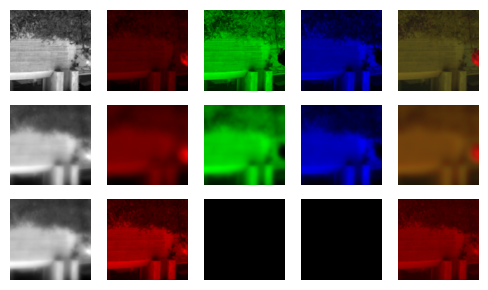
\includegraphics[width=0.9\textwidth]{figs/ClassicUnetSSIM_LR/pixel_comparison/4423_test3_ssim.png}
    \caption{Comparison of Pseudo-RGB images between ground truth (top row), hyperspectral blurred images (middle row), and the HyperUnet\textsubscript{SSIM}} outputs.
    \label{fig:degeneration_mode}
\end{figure}

\begin{figure}[!htb]
    \centering
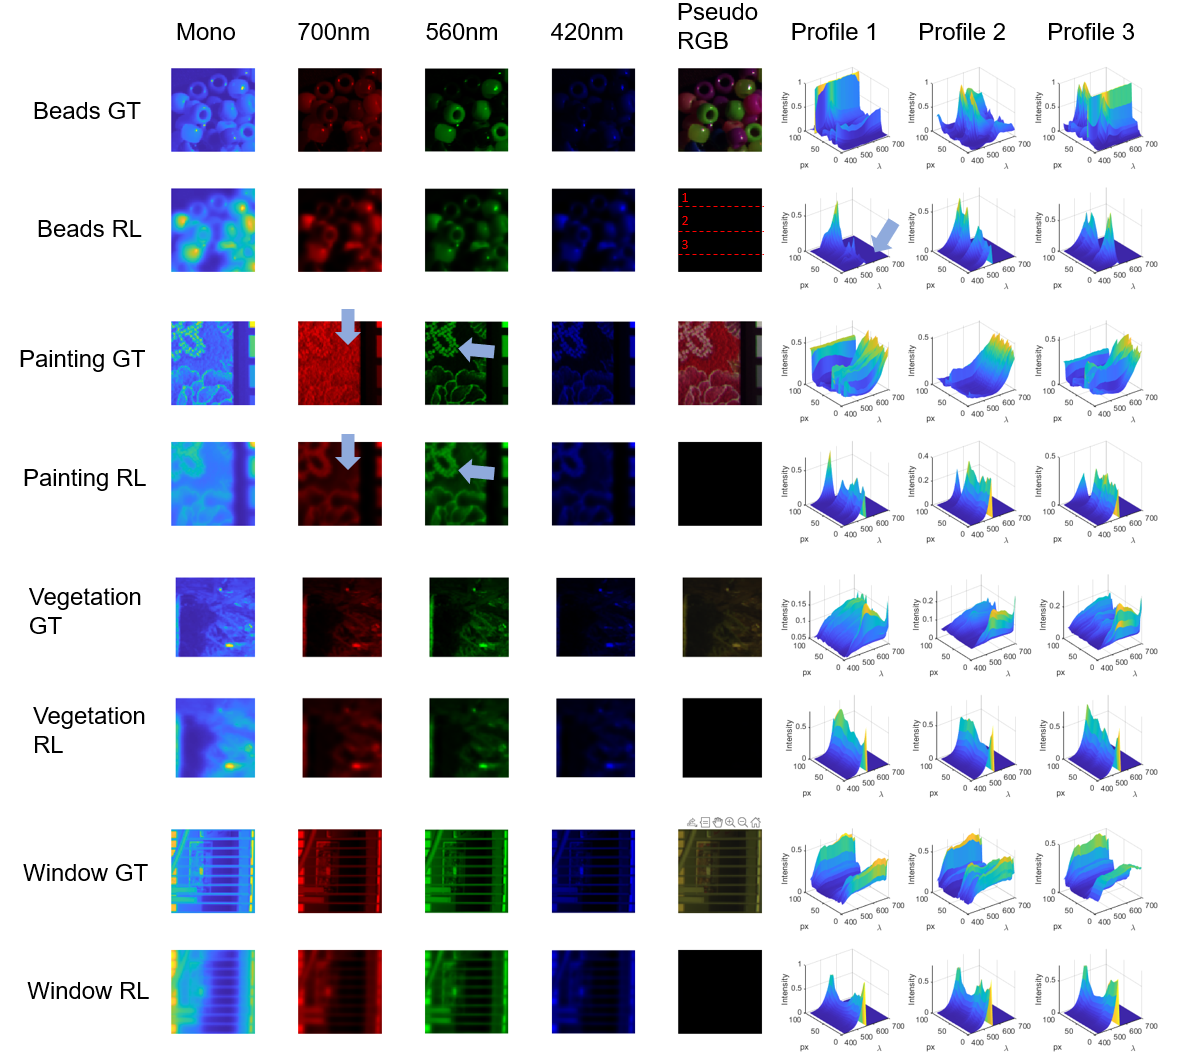
\includegraphics[width=\textwidth]{figs/RL/RLcompare.png}
    \caption{Pixel comparison between Ground Truth and Predicted test images for 3D RL.}
    \label{fig:RLCompare}
\end{figure}

\begin{figure}[!htb]
    \centering
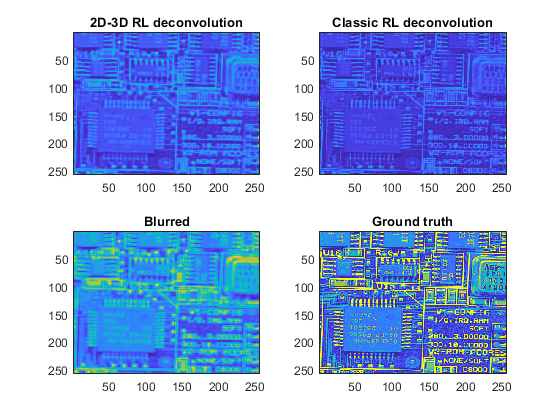
\includegraphics[width=\textwidth]{figs/RL/2D_RLcompare.png}
    \caption{Comparison of 2D-3D and Classic RL deconvolution results. The images from top to bottom for each respective side is a comparison between ground truth and predicted test images.}
    \label{fig:RL2DCompare}
\end{figure}

\begin{figure}[!htb]
    \centering
    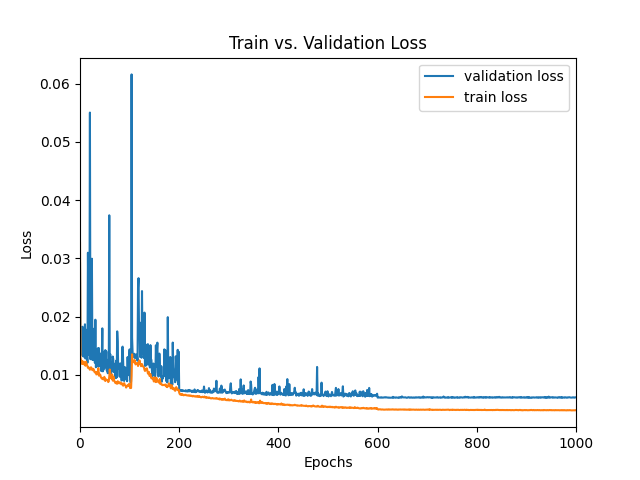
\includegraphics[width=\textwidth]{figs/ReducedUnet/loss_curves/loss_curve.png}
    \caption{Loss curve of ReducedUnet Architecture. This was done as an exploration of the overfitting issue seen in previous models and also because of the limited time and computing resources available.}
    \label{fig:loss_curve_ReducedUnet_model}
\end{figure}
\begin{figure}[!htb]
    \centering
    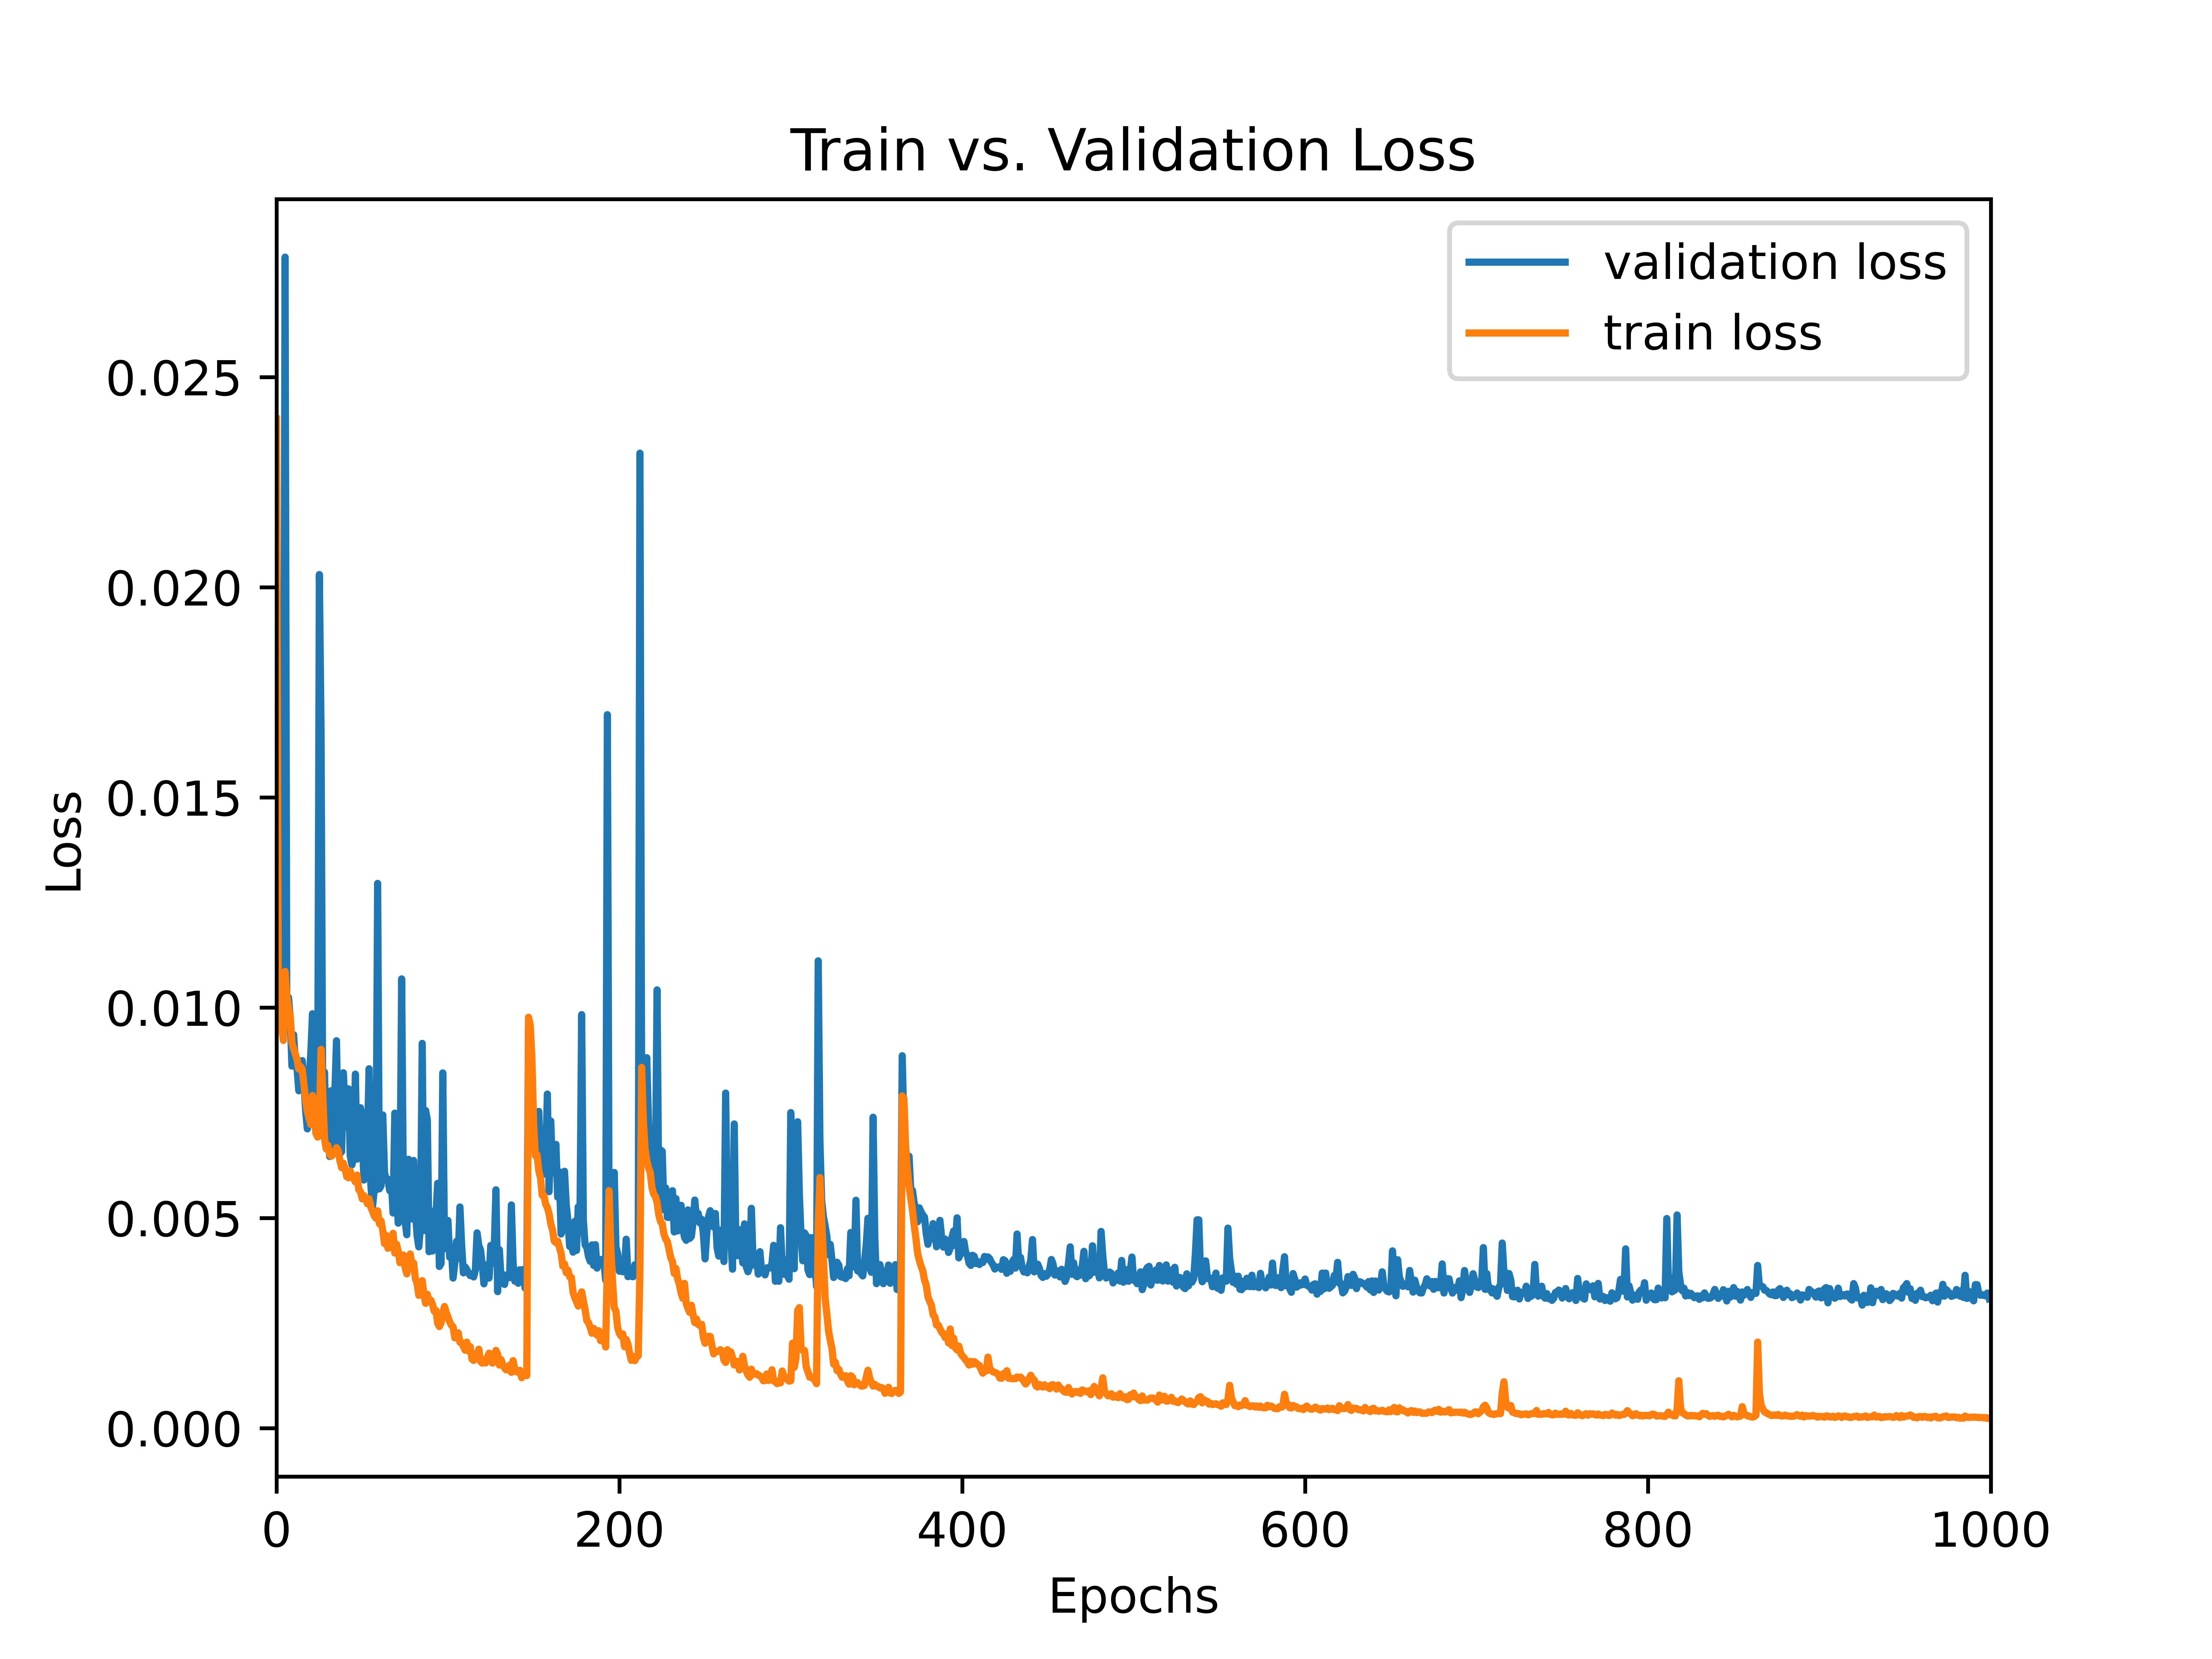
\includegraphics[width=\textwidth]{figs/ClassicUnet/curves/loss_curve.png}
    \caption{Loss curve for HyperUnet.}
    \label{fig:loss_curve_HyperNet_model}
\end{figure}

\begin{figure}[!htb]
    \centering
    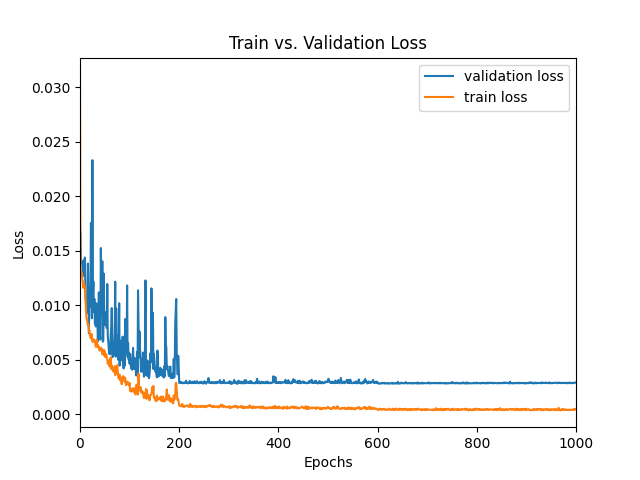
\includegraphics[width=\textwidth]{figs/ClassicUnet_LR/curves/loss_curve.png}
    \caption{Loss curve for HyperUnet\textsubscript{LR}.}
    \label{fig:loss_curve_HyperNetLR_model}
\end{figure}

\begin{figure}[!htb]
    \centering
    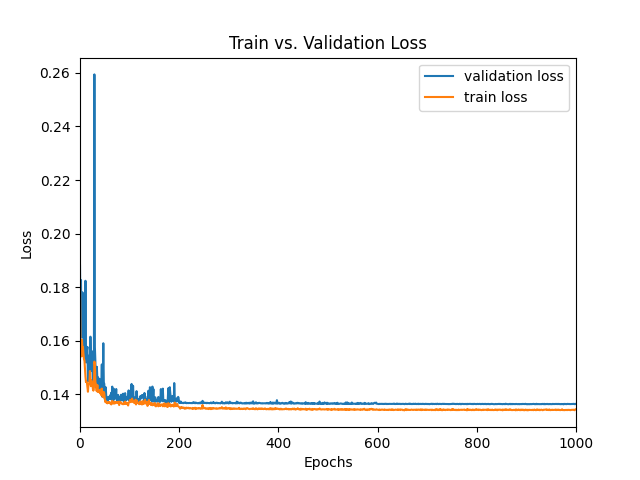
\includegraphics[width=\textwidth]{figs/ClassicUnetSSIM_LR/curves/loss_curve.png}
    \caption{Loss curve for HyperUnet\textsubscript{SSIM}.}
    \label{fig:loss_curve_UnetSSIM_model}
\end{figure}

\begin{figure}[!htb]
    \centering
    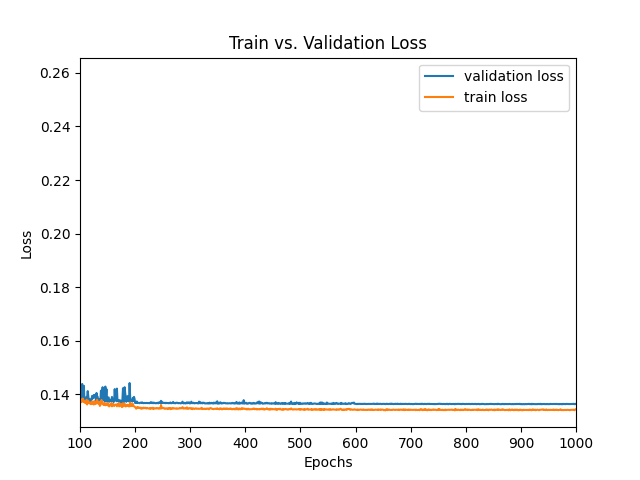
\includegraphics[width=\textwidth]{figs/ClassicUnetSSIM_LR/curves/loss_curve_zoom.png}
    \caption{Loss curve for HyperUnet\textsubscript{SSIM}: 100-200 epochs.}
    \label{fig:loss_curve_UnetSSIMzoom_model}
\end{figure}

\begin{figure}[!htb]
    \centering
    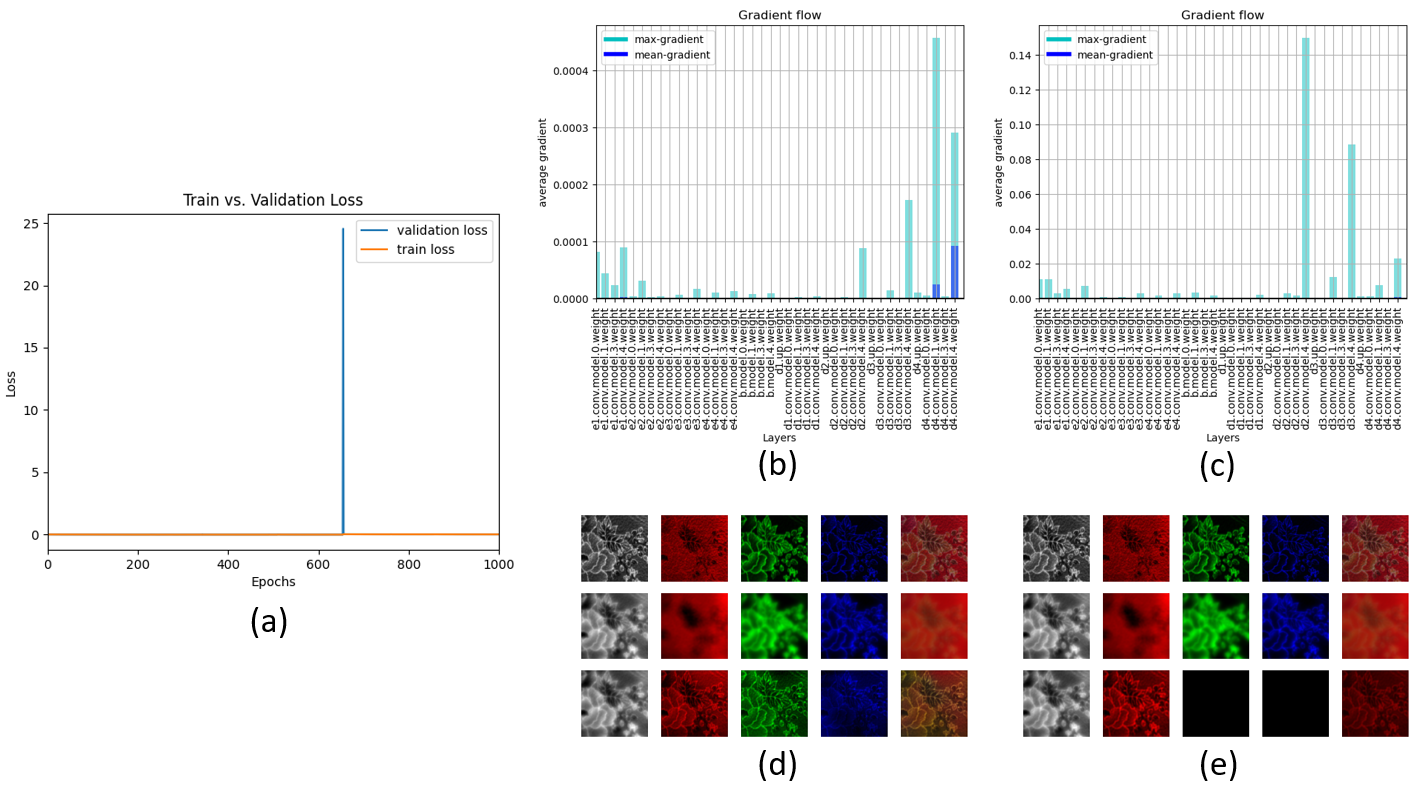
\includegraphics[width=\textwidth]{figs/loss_curve.png}
    \caption{Loss curve for a degenerate model that experienced extreme instability in training.}
    \label{fig:loss_curve_unstable}
\end{figure}

\begin{figure}[!htb]
    \centering
    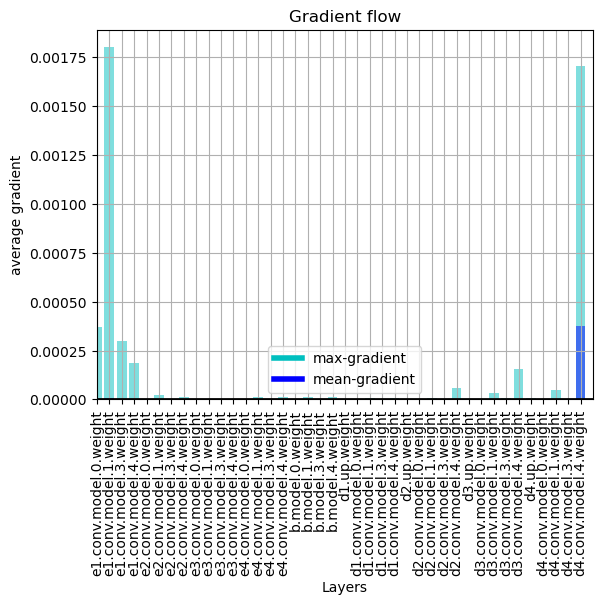
\includegraphics[width=\textwidth]{figs/ClassicUnet_LR/grads/grads999.png}
    \caption{Gradient size plots for HyperNet\textsubscript{LR}.}
    \label{fig:UnetLR_grads}
\end{figure}

\begin{figure}[!htb]
    \centering
    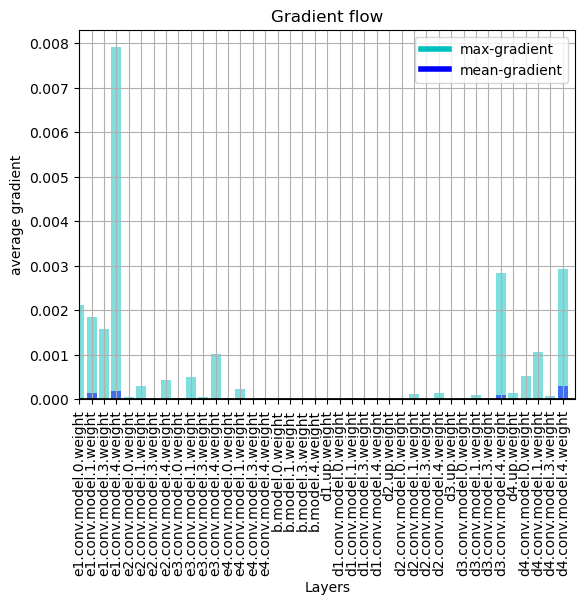
\includegraphics[width=\textwidth]{figs/ClassicUnetSSIM_LR/grads/grads999.png}
    \caption{Gradient size plots for HyperNet\textsubscript{SSIM}.}
    \label{fig:UnetSSIM_grads}
\end{figure}

\end{document}